\chapter{Service-oriented computing}
\label{chap:service-oriented computing}
\emph{Service-oriented computing} represents a distributed computing platform \cite{soa-contract}. It has its own paradigm, logic, architecture and patterns. It is built on the idea of distributed computing platforms and extends it by new considerations about governance, design layers and technologies suitable for its implementation.


\emph{Service orientation} is a design paradigm. It provides separation into logical units which can be utilized according to strategic goals and benefits of a requested target.

\section{Service-oriented architecture}
\emph{Service-oriented architecture (SOA)} is a set of best practices for an organization moving towards \gls{agile} architectural model of the system to meet business needs. Result of applied practices is an architecture which corresponds to dynamic market changes. The SOA best practices describe the human behaviour. There is no list of constraints which have to be followed in order to obtain a service-oriented architecture. The best practices are designed to resolve specific situations which the organization can meet. Depending on them just a subset of appropriate practices which are necessary to apply could be selected.\par

The architecture is layered. Layers can be multiple and can differ according to needs of designed system. One of the examples of horizontal layers is shown in Figure \ref{fig:soa-architecture}. The layers are separated and each of them encapsulates its implementation so that another layer can't access and modify it (preventing potential harms). In this example is an application containing services which have access to a database using an adapter. The \textit{\gls{adapter}} serves to transform data from database to data useful for services and vice-versa. \textit{Services} are entry point for consumer's application. They provide access to the data without direct access to \textit{database}.

One of the main advantages of a service-oriented architectural style is its ability to efficiently deal with changes. \textit{"SOA is based on a decomposition of enterprise IT assets and separation of 'stable' IT artifacts (services) from 'changeable' artifacts (business processes), orchestrating services into IT solutions (processes)."} \cite{website:versioning-in-soa}. %(http://msdn.microsoft.com/en-us/library/bb491124.aspx) 

Above mentioned services are essential part of SOA. Relations between them and a business process constituted by services are visualized in Figure \ref{fig:business-process-services}. The business process is a process from the real world whose workflow is simulated by services. A single task of business process is composed by one or more of the services. Services perform the logic, comunicate with underlying layers to retrieve and store data to operate as a business process.

\begin{figure}[htp] \centering{
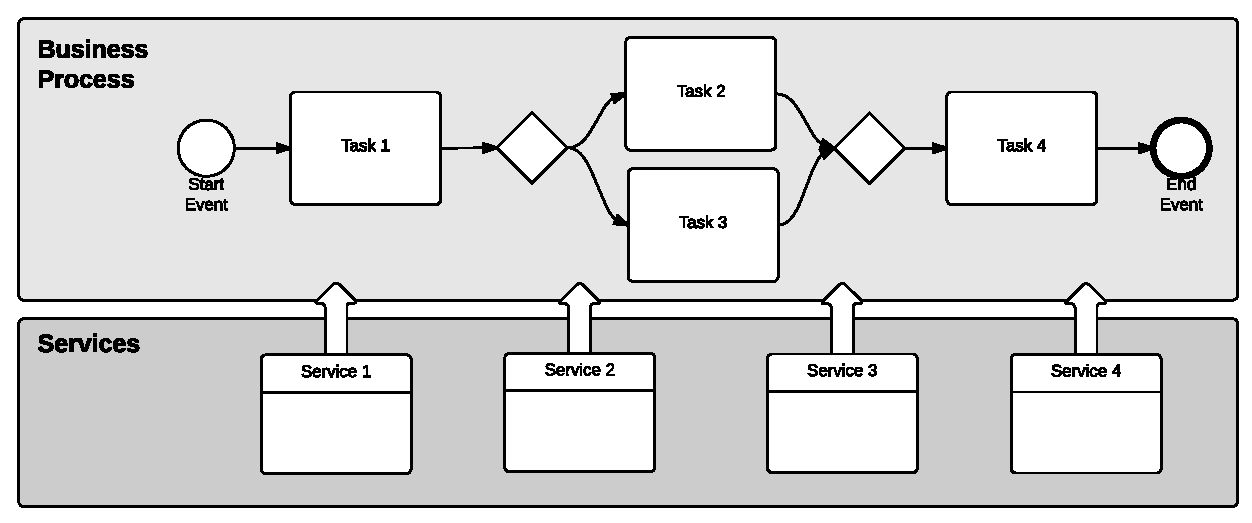
\includegraphics[width=12cm]{img/business-process-services.pdf}}
\caption{Business process is a composition of services}
\label{fig:business-process-services}
\end{figure} 

The speed of changes in the business is too fast to be passed directly into development and maintenance of a \gls{monolithic-systems}. Functionality of these systems is based on measures of customer and often can't deal with changes easily, it interfere in design of the whole architecture. SOA offers better flexibility when business requirements change. Changes are reflected into modifications of an existing business process by changing involved services or if it's needed a whole new process is created using existing services. When the existing services do not meet the requirements a new service can be created. There are more approaches how to deal with the changes and one of them is versioning which is described in Chapter \ref{chap:versioning} and Chapter \ref{chap:versionaccess} in detail.

\section{Services}
\label{sec:services}
\gls{service-oriented-design} is composed from logic units - services. Every service is a standalone object or component. Every service has its own functional context and related capabilities. Each service is deployed independently on other ones and on the system which uses it. It allows a parallel development, one service can be a part of many products of a corporation.
\textit{"The essence of Service in the SOA context is the business abstraction - that is a representation of functionality and/or data presented in business context."} \cite{agile-architecture}

\subsection{Service lifecycle}
\label{subsec:lifecycle}
The lifecycle of the services pass through several stages. Firstly the business which has to be abstracted by services is analysed. It is defined a set of services and compositions of services abstracting business processes. Than the services cen be designed, implemented and tested to work as expected. After that they are deployed and put into use of consumer. Deployed and consumed services are maintained by provider, moreover they are monitored. Monitoring helps to improvement of services. Finally services are versioned. A new version of a service can be implemented than the old one is retired.

Service lifecycle stages \cite{soa-governance}:
\begin{enumerate}
  \item Service-oriented ananlysis \\
  During this phase the services candidates, their capabilities and compositions are created. The analysis is typically interative, for each business process a service inventory is created.
  \item Service-oriented design \\
  This stage designs the service contracts. For every service candidate it is considered a technical contract, in case of REST services (described in Chapter \ref{chap:rest}). It is inevitable to think of HTTP methods usage, resource identifiers and header parameters.
  \item Serivce Logic Design \\
  During this phase the service architecture and its logic is established, so that the service will carry out the functionality which results from the contract.
  \item Service Development \\
  The implementation of the services is performed. It is based on the specifications and architecture design from previous stages.
  \item Service Testing \\
  The implemented services need to be tested in order to provide the quality assurance of developed application.
  \item Service Deployment and Maintenance \\
  In this phase the services are deployed on production environment. Maintenance involves changes and upgrades of services related to production environment, but it doesn't include changes which would result in new version of services.
  \item Service Usage and Monitoring \\
  Deployed service which is in use is an object of monitoring. It is essential for obtaining various metrics. Measured values can positively influence the maintenance and are further used for business assessment.
  \item Service Discovery \\
  Process of identifying \gls{agnostic-services} throughout the given service inventory.
  \item Service Versioning and Retirement \\
  After deployment and usage a need to change the logic of a service or addition of a new one can arise. Addition of new service version occures. How to version the services will be explained in Chapter \ref{chap:versioning}. 
  
  Retirement encompasses the termination of a service usage. Regarding service versioning a version of service which is no longer in use can be retired.
\end{enumerate}

\subsection{Levels of a service} 
\label{subsec:levels-of-service}

It is not completely clear what a service represets. It was already mentioned it is an an abstraction of business process but after all analysis stage it is implemented and represented by code.
In fact there are three levels of how the word \emph{Service} can be interpreted in SOA context \cite{agile-architecture}:
\begin{enumerate}
  \item \textbf{Service implementation} \hfill \\
Service implementation is the code containing the logic.
  \item \textbf{Service interface} \hfill \\ 
This level is an entry point to the service implementation, it provides underlying logic to consumers but encapsulating it in a way that consumers can see the implementation. 
  \item \textbf{Abstracted service} \hfill \\
Abstracted service or business service represents a business capability or data. A composition of services describe a business process. This is a core abstraction of SOA.
\end{enumerate}

There is a many-to-many relationship between these three levels. Business service can represents multiple interfaces and in the same time one interface can be supported by multiple implementation.

%TODO picture of service levels

%\subsection{Service categories and types} 

%There are two main types of services. The first type is composed by infrastructural services which provide the facilities and aren't a part of application. To the second type belongs services which are the part of the application and provide main logic.

\bigskip
%TODO describe services

%Service categories \cite{website:ontology-taxonomy} :
%\begin{description}
 % \item[Bus services] can be further divided into 
  %\begin{enumerate}
   % \item Communication services 
    %\item Utility services
  %\end{enumerate}
  %\item[Application services] consist of   
  %\begin{enumerate}
   % \item Entity services
    %\item Capability services
    %\item Activity services
    %\item Process services
  %\end{enumerate}
%\end{description}

%TODO image 

\section{Web services}
Web services are one group of services, these are intended to work on a network such as the Internet.

/TODO write shortly about RCP, WSDL, SOAP
%TODO form agile architecture revolution
 
\subsubsection{REST}
%TODO WADL ??

Representational State Transfer, REST is an architectural style for building distributed hypermedia applications. This thesis deals with REST architectural style and REST services. They will be described in detail within the next chapter. \ref{chap:rest}

\section{Service granularity}
\label{sec:granularity}
In SOA context granularity is an often used expression. Granularity of an entity represents amount of data which is understood as one unit related to the whole data pool. It is possible to distinguish from fine-grained to coarse-grained granularity. Where fine-grained contains small amount of data in one unit respective to whole data pool. On the contrary the coarser granularity bears much more data in one unit.

Service granularity is defined during analytical part of the service design. Granularity determines properties of the services related to the business process. Services can be fine-grained up to coarse-grained. When services are fine-grained number of services is higher and they contain less logic. Therefore the cost of the implementation is smaller and the higher reusability is provided. However the effort needed to compose these services into a process is higher. 

On the other side when services are coarse-grained they contain more complex logic and easily compose the process. However reusability is limited and more effort is required to implement them.

The example of fine-grained and coarse-grained granularity can be shown on the business process of ordering a product.

The coarse-grained service would contained more logic. It can be responsible for whole order. The service would execute the product selection, delivery address submittion, choice of delivery option and payment option. Having one service to order the product offer less interactions between client and server. However the service is less flexible because of fixed steps of ordering. If there was a need to add a one step into the ordering process the service would have to be changed.

On the other side the order process could be composed by fine-grained services. One service is responsible just for one of the actions. Order is than a composition of Products, Addresses, DeliveryOptions and PaymentsOptions services. The services are flexibly composed to perform the ordering process. If there was a need to add an additional step in the process there would be added a new service with this logic.





%%\subsubsection*{\textbf{Guacamole} \hfill \emph{http://guac-dev.org/}}
%%\label{subsec:guacamole}
%% \ref{}.
%%    \item \textbf{[název předmětu 1]} \hfill \\
%%    odkaz na stránku předmětu, obsahující pouze název a informace o spolufinancování \gls{eu}
    
%%\begin{table}
%%  \caption{Základní typy entit v Drupalu}
  %%\label{tab:typy-entit}
  %%\begin{tabular}{ | p{3cm} | l | c | c | }
   %% \hline 
    %%Typ entity & Strojový název & Dostupnost polí & Rozšiřitelnost \\ \hline 
    %%Komentář & comment & \checkmark & \checkmark \\ \hline 
    %%Soubor & file &  & \\ \hline 
    %%Slovník & vocabulary &  & \\ \hline 
    %%Uzel & node & \checkmark & \checkmark \\ \hline 
    %%Uživatel & user & \checkmark & \checkmark \\ \hline 
    %%Záznam slovníku & term & \checkmark & \checkmark \\ \hline             
  %%\end{tabular}
%%\end{table}
%% \emph \emph \texttt.
